\begin{figure}[H]
  \centering
  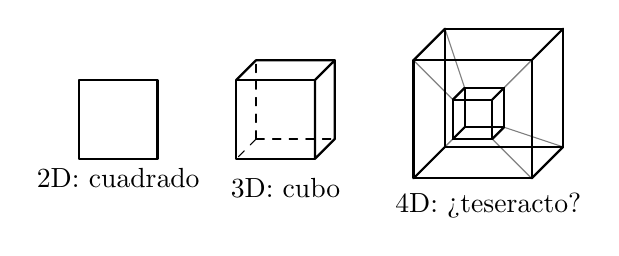
\begin{tikzpicture}[scale=0.5,line join=round,line cap=round,x=1cm,y=1cm]
    \begin{scope}[shift={(0,0)}]
      \draw[thick] (0,0) rectangle (2,2);
      \node at (1,-0.5) {2D: cuadrado};
    \end{scope}

    \begin{scope}[shift={(4,0)}]
      % Hidden edges
      \draw[dashed] (0.5,0.5) -- (2.5,0.5);
      \draw[dashed] (0.5,0.5) -- (0.5,2.5);
      \draw[dashed] (0.5,0.5) -- (0,0);
      
      % Visible faces
      \draw[thick] (0,0) rectangle (2,2);
      \draw[thick] (2,0) -- (2.5,0.5) -- (2.5,2.5) -- (2,2) -- cycle;
      \draw[thick] (0,2) -- (0.5,2.5) -- (2.5,2.5);
      
      \node at (1.25,-0.75) {3D: cubo};
    \end{scope}

    \begin{scope}[shift={(9,0)}]
      % Inner cube (smaller)
      \coordinate (A1) at (0.5,0.5); \coordinate (B1) at (1.5,0.5);
      \coordinate (C1) at (1.5,1.5); \coordinate (D1) at (0.5,1.5);
      \coordinate (A2) at (0.8,0.8); \coordinate (B2) at (1.8,0.8);
      \coordinate (C2) at (1.8,1.8); \coordinate (D2) at (0.8,1.8);

      % Outer cube (larger)
      \coordinate (E1) at (-0.5,-0.5); \coordinate (F1) at (2.5,-0.5);
      \coordinate (G1) at (2.5,2.5);   \coordinate (H1) at (-0.5,2.5);
      \coordinate (E2) at (0.3,0.3);   \coordinate (F2) at (3.3,0.3);
      \coordinate (G2) at (3.3,3.3);   \coordinate (H2) at (0.3,3.3);

      % Connecting inner and outer vertices
      \foreach \from/\to in {A1/E1, B1/F1, C1/G1, D1/H1, A2/E2, B2/F2, C2/G2, D2/H2}
        \draw[gray, thin] (\from) -- (\to);

      % Draw Inner Cube
      \draw[thick] (A1) -- (B1) -- (C1) -- (D1) -- cycle;
      \draw[thick] (A2) -- (B2) -- (C2) -- (D2) -- cycle;
      \foreach \from/\to in {A1/A2, B1/B2, C1/C2, D1/D2} \draw[thick] (\from) -- (\to);

      % Draw Outer Cube
      \draw[thick] (E1) -- (F1) -- (G1) -- (H1) -- cycle;
      \draw[thick] (E2) -- (F2) -- (G2) -- (H2) -- cycle;
      \foreach \from/\to in {E1/E2, F1/F2, G1/G2, H1/H2} \draw[thick] (\from) -- (\to);

      \node at (1.4,-1.2) {4D: ¿teseracto?};
    \end{scope}
  \end{tikzpicture}
\end{figure}